\section{Experiments and Results}

We ran several experiments to test the model's ability for binary RTP/non-RTP detection as well as multi-class protocol identification. All tests were performed on a single CPU of a 1.6 GHz dual-core Intel i5 processor with 16 GB DDR3 RAM. In the binary confusion matrix, true positive (TP) indicates correct classification of data. True negative (TN) is correct classification of data as non-RTP. false negative (FN) implies incorrect identification of traffic as non-RTP, and false positive (FP) is the incorrect classification of data as RTP. We use measurements of precision, recall, and F1-score for model evaluation, defined as follows:

\begin{equation}
\begin{split}
    Recall = \frac{TP}{TP + FP} \text{  }
    Precision = \frac{TP}{TP + FN} \\
    F1\text{ }Score = \frac{2(P\times R)}{P + R} \\
    \end{split}
\end{equation}

\subsection{RTP Detection}

For the binary RTP/non-RTP classification, we merged SRTP and RTP traffic into an RTP label and re-labeled all non-RTP and non-SRTP traffic as non-RTP. For testing the different configurations of the \textsc{Maple} model, we first processed traffic and transformed it into a matrix image, and then used it as input for each of the models. We performed random under-sampling to avoid bias in the dataset, and then split the data into 60\%/40\% for training and testing. We ran the multi-model using \textsc{Alpine} and \textsc{Palm} with the same datasets with the results in Table~\ref{tab:rtpresultslsh} to establish a baseline for comparison. Then we ran tests with training for $3$ epochs for each CNN model. As we plan to deploy this technology in a real RTP detection and deep packet inspection system, we also measured classification throughput in order to determine how much traffic the \textsc{Maple} system would be able to process given the detection model configuration. Results are provided in Table~\ref{tab:binaryresults}.

\begin{table} [h!]
\centering
\begin{tabular}{| r | c | c | c |}
\hline
Class & P & R & F1 \\
\hline
\textit{Non-RTP} & 0.73 & 0.77 & 0.75 \\
\textit{RTP} & 0.76 & 0.71 & 0.73 \\
\hline
\end{tabular}
\caption{Classification results of RTP vs non-RTP detection for the LSH model}
\label{tab:rtpresultslsh}
\end{table}

\begin{table} [h!]
\centering
\small
\begin{tabular}{| r | c | c | c |}
\hline
Model & P & R & F1 \\
\hline
\textbf{A} &&& \\
\textit{Non-RTP} & 0.96 & 0.99 & 0.98 \\
\textit{RTP} & 0.99 & 0.96 & 0.98 \\
\hline
\textbf{B} &&& \\
\textit{Non-RTP} & 0.97 & 0.99 & 0.98 \\
\textit{RTP} & 0.99 & 0.97 & 0.98 \\
\hline
\textbf{C} &&& \\
\textit{Non-RTP} & 1.00 & 0.99 & 1.00 \\
\textit{RTP} & 0.99 & 1.00 & 1.00 \\
\hline
\textbf{D} &&& \\
\textit{Non-RTP} & 1.00 & 1.00 & 1.00 \\
\textit{RTP} & 1.00 & 1.00 & 1.00 \\
\hline
\textbf{E} &&& \\
\textit{Non-RTP} & 1.00 & 1.00 & 1.00 \\
\textit{RTP} & 1.00 & 1.00 & 1.00 \\
\hline
\end{tabular}
\caption{Classification results of RTP vs non-RTP detection for all \textsc{Maple} models}
\label{tab:binaryresults}
\end{table}

\begin{table}
\centering
\small
\begin{tabular}{| r | c | c |}
\hline
Model & Accuracy & Mb/s \\
\hline
\textbf{A} & 0.975348 & 12.5 \\
\hline
\textbf{B} & 0.978258 & 9.28 \\
\hline
\textbf{C} & 0.996934 & 7.07 \\
\hline
\textbf{D} & 0.995908 & 10.41 \\
\hline
\textbf{E} & 0.996847 & 5.3 \\
\hline
\end{tabular}
\caption{Throughput results of RTP vs non-RTP detection for all \textsc{Maple} models}
\label{tab:binarythroughput}
\end{table}

Generally, the ResNet model performed exceedingly well at the RTP detection task, exceeding ninety-nine percent accuracy across all the configurations. The LeNet models performed marginally worse in terms of accuracy, but the smaller of the two models had the highest throughput of any of the tested configurations. Another configuration choice which may have significant impact on model accuracy is the number of epochs trained. Real systems place an emphasis on minimizing down time of a system, but in actual deployment many models may be trained offline and then embedded. In systems where training time is not a factor of performance, we can thus increase the number of epochs with little real impact. In order to test the efficacy of such a design choice, we re-ran \textsc{Maple} models A and C with 10 epochs to see if performance improved. Results in Tables~\ref{tab:addepoch1} and ~\ref{tab:addepoch2} show that ResNet appears to learn faster than LeNet, as it gained very little improvement with additional training time. Interestingly, with additional training time LeNet approaches similar accuracy to ResNet but still maintains higher throughput.

\begin{table} [h!]
\centering
\small
\begin{tabular}{| r | c | c | c |}
\hline
Model & P & R & F1 \\
\hline
\textbf{A} &&& \\
\textit{Non-RTP} & 0.99 & 0.99 & 0.99 \\
\textit{RTP} & 0.99 & 0.99 & 0.99 \\
\hline
\textbf{C} &&& \\
\textit{Non-RTP} & 1.00 & 1.00 & 1.00 \\
\textit{RTP} & 1.00 & 1.00 & 1.00 \\
\hline
\end{tabular}
\caption{Classification results of RTP vs non-RTP detection for \textsc{Maple} models A and C with additional training time}
\label{tab:addepoch1}
\end{table}

\begin{table} [h!]
\centering
\small
\begin{tabular}{| r | c | c |}
\hline
Model & Accuracy & Mb/s \\
\hline
\textbf{A} & 0.990499 & 14.99 \\
\hline
\textbf{C} & 0.998172 & 7.38 \\
\hline
\end{tabular}
\caption{Throughput results of RTP vs non-RTP detection for \textsc{Maple} models A and C with additional training time}
\label{tab:addepoch2}
\end{table}

\subsection{Protocol Auto Detection}

As previously mentioned, many middlebox technologies are interested in multi-classification problems where many different applications or protocols need to be identified. Thus, we expand our experiments to a 26-protocol problem using the combined dataset described in chapter 4. We again use models A and C, LeNet and ResNet respectively, for this expansion. As this is a much harder problem, we expect to need more training time. We ran each model with 10 epochs and 50 epochs, and recorded the macro averages in Table~\ref{tab:multiresults}.

\begin{table} [h!]
\centering
\begin{tabular}{| r | c | c | c | c |}
\hline
Model & P & R & F1 & Accuracy \\
\hline
\textbf{A - 10 epochs} & 0.78 & 0.78 & 0.77 & 0.780920\\
\textbf{50 epochs} & 0.83 & 0.83 & 0.83 & 0.832446 \\
\hline
\textbf{C - 10 epochs} & 0.84 & 0.84 & 0.83 & 0.835993 \\
\textbf{50 epochs} & 0.86 & 0.85 & 0.85 & 0.849528\\
\hline
\end{tabular}
\caption{Results of multi-class detection for models A and C as macro averages}
\label{tab:multiresults}
\end{table}

Increasing the training time for the LeNet model showed significant improvement in accuracy, but not likely to a level needed for deployed systems so there is a need to build upon the baseline. The ResNet model approaches better accuracy with more training time.

\subsection{User Fingerprinting}
In order to test capability to track user streams, we isolated a source/destination IP pair in the traffic and created a separate user label for it. In this way, we associate a particular traffic stream with a person of interest. Then, we configured \textsc{Maple} and a multimodal version of \textsc{Alpine} to use no network layer features, and instead rely on packet length, flags, and analysis of payload contents and spatial features to make the classification. Results in Figure~\ref{fig:userbob} show this approach as a promising solution for tracking user streams across changing network configurations.

\begin{figure} [ht!]
\centering
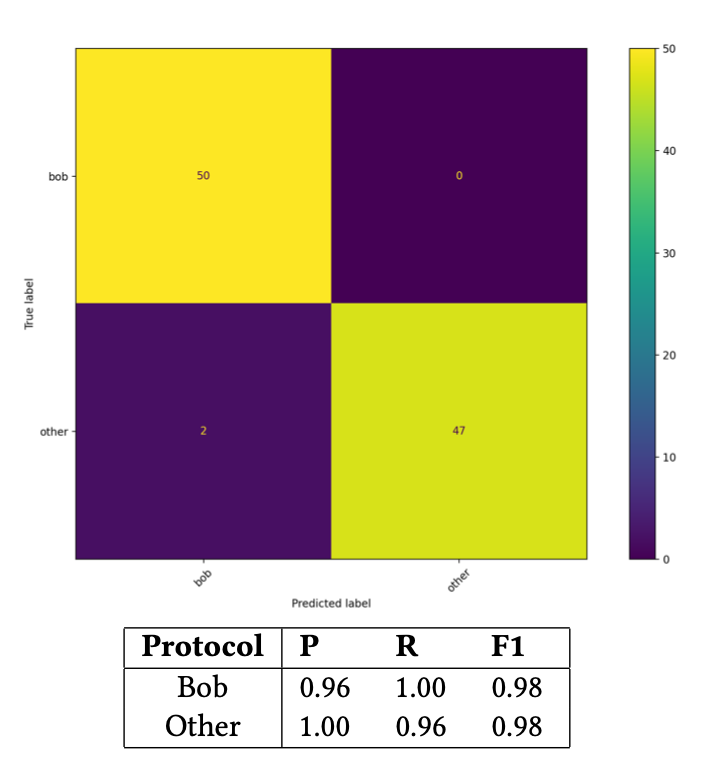
\includegraphics[scale=0.7]{chapters/5/img/userbob.png}
\caption{A confusion matrix of tracking user Bob across traffic streams in a changing network environment}
\label{fig:userbob}
\end{figure}

\subsection{Model Performance and Throughput}
Decreasing the number of kernels may have slightly impacted accuracy, but improved overall throughput significantly and lessens memory footprint. In a real network environment, it may be worth consideration to sacrifice some accuracy in order to be able to monitor more traffic or more effectively load-balance the received input depending on hardware capability. Thus, the ideal model configuration is often environment-dependent and inspired us to incorporate configuration capability in \textsc{Maple} so that the deployed system may best suit the environment. We provide the throughput of each model configuration in our experiments in Table~\ref{tab:binarythroughput}.
